% Options for packages loaded elsewhere
\PassOptionsToPackage{unicode}{hyperref}
\PassOptionsToPackage{hyphens}{url}
%
\documentclass[
  english,
  man, donotrepeattitle,floatsintext]{apa7}
\usepackage{lmodern}
\usepackage{amssymb,amsmath}
\usepackage{ifxetex,ifluatex}
\ifnum 0\ifxetex 1\fi\ifluatex 1\fi=0 % if pdftex
  \usepackage[T1]{fontenc}
  \usepackage[utf8]{inputenc}
  \usepackage{textcomp} % provide euro and other symbols
\else % if luatex or xetex
  \usepackage{unicode-math}
  \defaultfontfeatures{Scale=MatchLowercase}
  \defaultfontfeatures[\rmfamily]{Ligatures=TeX,Scale=1}
\fi
% Use upquote if available, for straight quotes in verbatim environments
\IfFileExists{upquote.sty}{\usepackage{upquote}}{}
\IfFileExists{microtype.sty}{% use microtype if available
  \usepackage[]{microtype}
  \UseMicrotypeSet[protrusion]{basicmath} % disable protrusion for tt fonts
}{}
\makeatletter
\@ifundefined{KOMAClassName}{% if non-KOMA class
  \IfFileExists{parskip.sty}{%
    \usepackage{parskip}
  }{% else
    \setlength{\parindent}{0pt}
    \setlength{\parskip}{6pt plus 2pt minus 1pt}}
}{% if KOMA class
  \KOMAoptions{parskip=half}}
\makeatother
\usepackage{xcolor}
\IfFileExists{xurl.sty}{\usepackage{xurl}}{} % add URL line breaks if available
\IfFileExists{bookmark.sty}{\usepackage{bookmark}}{\usepackage{hyperref}}
\hypersetup{
  pdftitle={Aggregation trial analysis},
  pdfauthor={Shir Dekel},
  pdflang={en-EN},
  hidelinks,
  pdfcreator={LaTeX via pandoc}}
\urlstyle{same} % disable monospaced font for URLs
\usepackage{graphicx,grffile}
\makeatletter
\def\maxwidth{\ifdim\Gin@nat@width>\linewidth\linewidth\else\Gin@nat@width\fi}
\def\maxheight{\ifdim\Gin@nat@height>\textheight\textheight\else\Gin@nat@height\fi}
\makeatother
% Scale images if necessary, so that they will not overflow the page
% margins by default, and it is still possible to overwrite the defaults
% using explicit options in \includegraphics[width, height, ...]{}
\setkeys{Gin}{width=\maxwidth,height=\maxheight,keepaspectratio}
% Set default figure placement to htbp
\makeatletter
\def\fps@figure{htbp}
\makeatother
\setlength{\emergencystretch}{3em} % prevent overfull lines
\providecommand{\tightlist}{%
  \setlength{\itemsep}{0pt}\setlength{\parskip}{0pt}}
\setcounter{secnumdepth}{-\maxdimen} % remove section numbering
% Make \paragraph and \subparagraph free-standing
\ifx\paragraph\undefined\else
  \let\oldparagraph\paragraph
  \renewcommand{\paragraph}[1]{\oldparagraph{#1}\mbox{}}
\fi
\ifx\subparagraph\undefined\else
  \let\oldsubparagraph\subparagraph
  \renewcommand{\subparagraph}[1]{\oldsubparagraph{#1}\mbox{}}
\fi
\raggedbottom
\usepackage{makecell}
\usepackage{enumitem}
\usepackage{pdflscape}
\usepackage{ntheorem}

% from https://tex.stackexchange.com/a/100907:
\newtheorem{hyp}{Hypothesis}

\makeatletter
\newcounter{subhyp}
\let\savedc@hyp\c@hyp
\newenvironment{subhyp}
 {%
  \setcounter{subhyp}{0}%
  \stepcounter{hyp}%
  \edef\saved@hyp{\thehyp}% Save the current value of hyp
  \let\c@hyp\c@subhyp     % Now hyp is subhyp
  \renewcommand{\thehyp}{\saved@hyp\alph{hyp}}%
 }
 {}
\newcommand{\normhyp}{%
  \let\c@hyp\savedc@hyp % revert to the old one
  \renewcommand\thehyp{\arabic{hyp}}%
}
\makeatother
% Manuscript styling
\usepackage{upgreek}
\captionsetup{font=singlespacing,justification=justified}

% Table formatting
\usepackage{longtable}
\usepackage{lscape}
% \usepackage[counterclockwise]{rotating}   % Landscape page setup for large tables
\usepackage{multirow}		% Table styling
\usepackage{tabularx}		% Control Column width
\usepackage[flushleft]{threeparttable}	% Allows for three part tables with a specified notes section
\usepackage{threeparttablex}            % Lets threeparttable work with longtable

% Create new environments so endfloat can handle them
% \newenvironment{ltable}
%   {\begin{landscape}\begin{center}\begin{threeparttable}}
%   {\end{threeparttable}\end{center}\end{landscape}}
\newenvironment{lltable}{\begin{landscape}\begin{center}\begin{ThreePartTable}}{\end{ThreePartTable}\end{center}\end{landscape}}

% Enables adjusting longtable caption width to table width
% Solution found at http://golatex.de/longtable-mit-caption-so-breit-wie-die-tabelle-t15767.html
\makeatletter
\newcommand\LastLTentrywidth{1em}
\newlength\longtablewidth
\setlength{\longtablewidth}{1in}
\newcommand{\getlongtablewidth}{\begingroup \ifcsname LT@\roman{LT@tables}\endcsname \global\longtablewidth=0pt \renewcommand{\LT@entry}[2]{\global\advance\longtablewidth by ##2\relax\gdef\LastLTentrywidth{##2}}\@nameuse{LT@\roman{LT@tables}} \fi \endgroup}

% \setlength{\parindent}{0.5in}
% \setlength{\parskip}{0pt plus 0pt minus 0pt}

% \usepackage{etoolbox}
\makeatletter
\patchcmd{\HyOrg@maketitle}
  {\section{\normalfont\normalsize\abstractname}}
  {\section*{\normalfont\normalsize\abstractname}}
  {}{\typeout{Failed to patch abstract.}}
\patchcmd{\HyOrg@maketitle}
  {\section{\protect\normalfont{\@title}}}
  {\section*{\protect\normalfont{\@title}}}
  {}{\typeout{Failed to patch title.}}
\makeatother
\shorttitle{}
\usepackage{csquotes}
\ifxetex
  % Load polyglossia as late as possible: uses bidi with RTL langages (e.g. Hebrew, Arabic)
  \usepackage{polyglossia}
  \setmainlanguage[]{english}
\else
  \usepackage[shorthands=off,main=english]{babel}
\fi

\title{Aggregation trial analysis}
\author{Shir Dekel\textsuperscript{}}
\date{}


\note{Created 2020-06-24 18:40:58}

\affiliation{\phantom{0}}

\begin{document}
\maketitle

\hypertarget{full-results}{%
\section{Full results}\label{full-results}}

The aggregation experiment includes a series of 10 separate investment decisions, and subsequently, 10 decisions presented on the same page (joint). Figure~\ref{fig:plot-full} shows proportions of project acceptance across all conditions and trials.

\begin{figure}
\centering
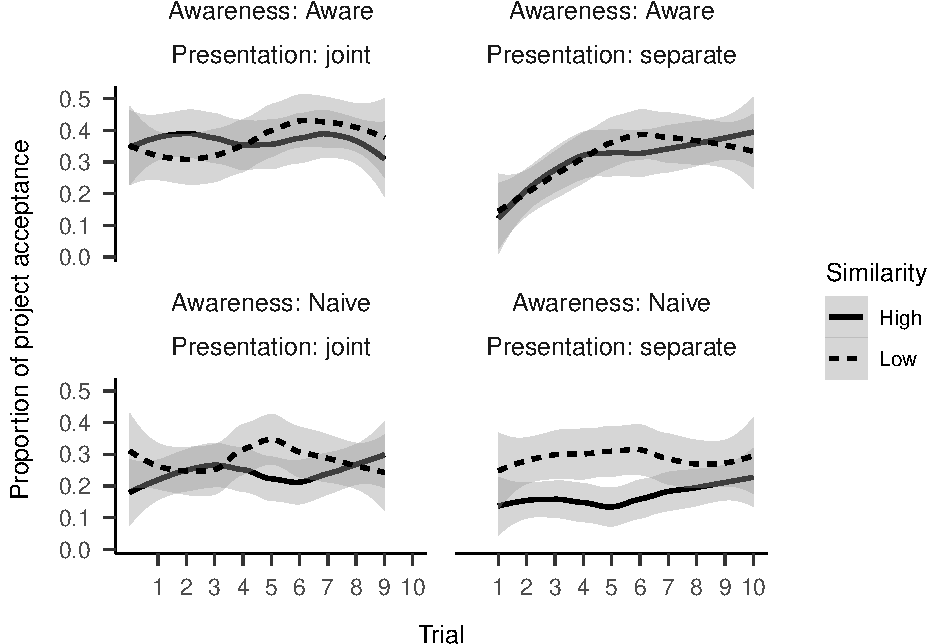
\includegraphics{aggregation_trials_files/figure-latex/plot-full-1.pdf}
\caption{\label{fig:plot-full}Proportion of project acceptance in the separate presentation condition, by trial, and similarity, awareness, and presentation conditions. The smoothing over trials is done using LOESS, and the shading represents 95\% confidence intervals.}
\end{figure}

\hypertarget{results-of-interest}{%
\section{Results of interest}\label{results-of-interest}}

The key findings seem to be in the separate presentation. As Figure~\ref{fig:plot-separate-trial-awareness} and Table~\ref{tab:separate-trial-awareness-tab} shows, in the separate condition people are more likely to accept projects over the 10 trials in the separate presentation, but this interacts with awareness. Specifically, the relationship between choice and trial is significant in the aware condition, \(b = 0.11\), \(t(1976) = 4.54\), \(p < 0.001\); but not in the naive condition, \(b = 0.03\), \(t(1976) = 1.01\), \(p = 0.31\).

\begin{figure}
\centering
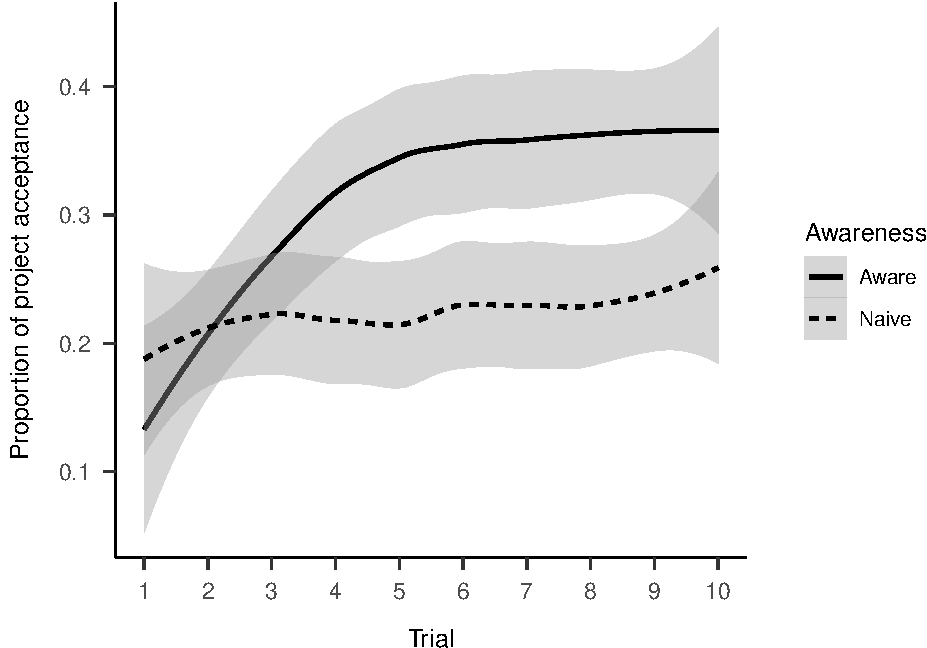
\includegraphics{aggregation_trials_files/figure-latex/plot-separate-trial-awareness-1.pdf}
\caption{\label{fig:plot-separate-trial-awareness}Proportion of project acceptance in the separate presentation condition, by trial and awareness conditions. The smoothing over trials is done using LOESS, and the shading represents 95\% confidence intervals.}
\end{figure}

\begin{table}[tbp]

\begin{center}
\begin{threeparttable}

\caption{\label{tab:separate-trial-awareness-tab}Logistic regression of project acceptance by order and awareness.}

\begin{tabular}{lllll}
\toprule
Predictor & \multicolumn{1}{c}{$b$} & \multicolumn{1}{c}{95\% CI} & \multicolumn{1}{c}{$z$} & \multicolumn{1}{c}{$p$}\\
\midrule
Intercept & -1.44 & $[-1.76$, $-1.14]$ & -9.09 & < .001\\
AwarenessNaive & 0.05 & $[-0.40$, $0.51]$ & 0.23 & .818\\
Order & 0.11 & $[0.06$, $0.16]$ & 4.54 & < .001\\
AwarenessNaive $\times$ Order & -0.08 & $[-0.15$, $-0.01]$ & -2.32 & .021\\
\bottomrule
\end{tabular}

\end{threeparttable}
\end{center}

\end{table}

\hypertarget{auto-correlations}{%
\section{Auto-correlations}\label{auto-correlations}}

A lag-1 auto-correlation calculates the correlation between a certain trial (usually a time point in time series data), and the trial before it. This is a measure of how dependent a series is on its past. For our purposes, a positive lag-1 autocorrelation would indicate more influence of bracketing, while a negative value would indicate more influence of diversification. Figures~\ref{fig:acf-separate-low},~\ref{fig:acf-separate-high},~\ref{fig:acf-joint-low}, and~\ref{fig:acf-joint-high} show the auto-correlations for the presentation and similarity conditions for the different lags. Looking only at lag-1, it seems as though for the separate presentation, both similarity conditions have positive lag-1 values, indicating bracketing. In the joint presentation, however, the values indicate a preference for bracketing in the low similarity condition, and a preference for diversification in the high similarity condition. However, I'm not yet sure how to compare these values statistically, so can not yet say whether these are significant.

\begin{figure}
\centering
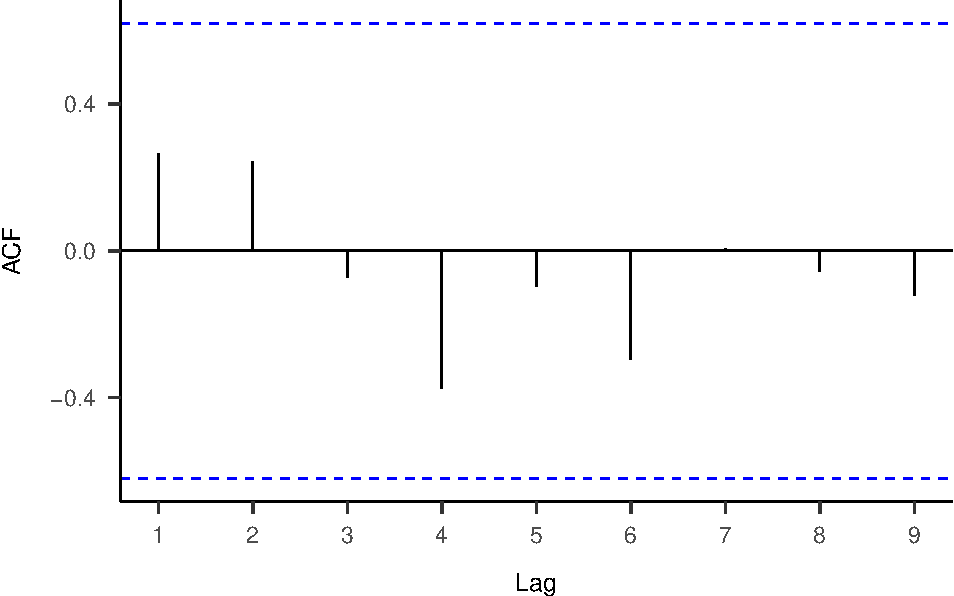
\includegraphics{aggregation_trials_files/figure-latex/acf-separate-low-1.pdf}
\caption{\label{fig:acf-separate-low}Autocorrelations of project acceptance proportions across trials, for the separate presentation low similarity condition. The dashed blue lines represent the 95\% CIs from zero.}
\end{figure}

\begin{figure}
\centering
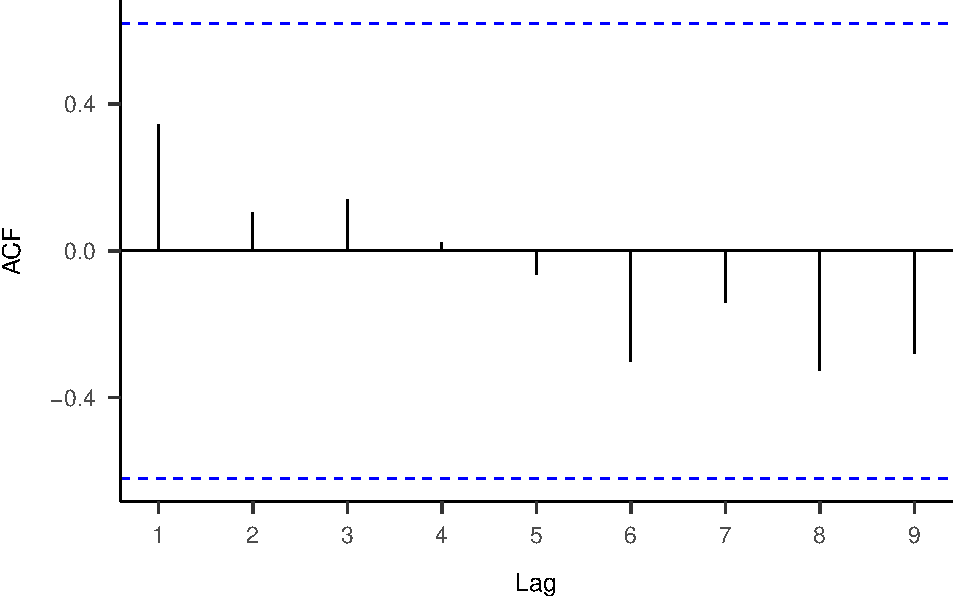
\includegraphics{aggregation_trials_files/figure-latex/acf-separate-high-1.pdf}
\caption{\label{fig:acf-separate-high}Autocorrelations of project acceptance proportions across trials, for the separate presentation high similarity condition. The dashed blue lines represent the 95\% CIs from zero.}
\end{figure}

\begin{figure}
\centering
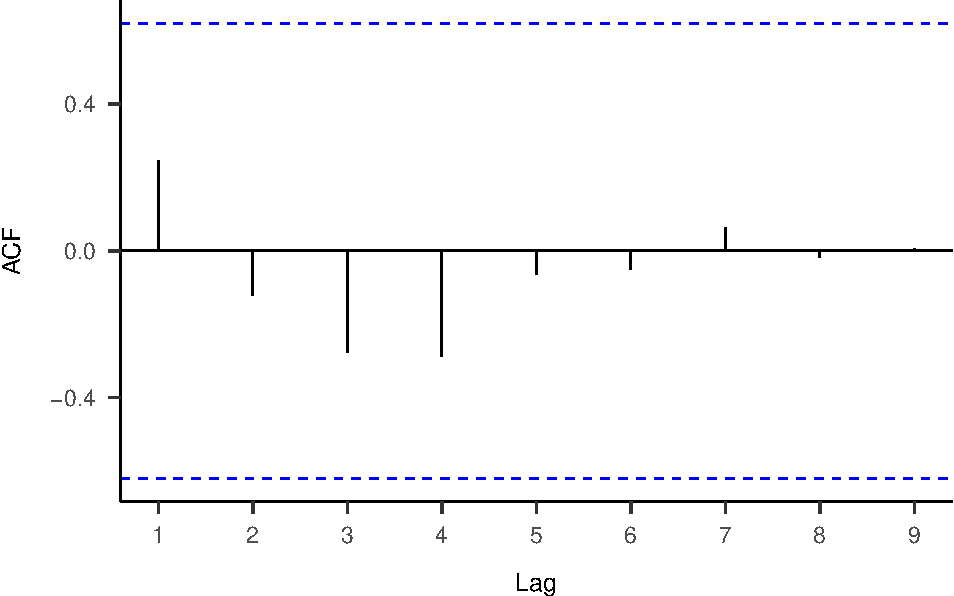
\includegraphics{aggregation_trials_files/figure-latex/acf-joint-low-1.pdf}
\caption{\label{fig:acf-joint-low}Autocorrelations of project acceptance proportions across trials, for the joint presentation low similarity condition. The dashed blue lines represent the 95\% CIs from zero.}
\end{figure}

\begin{figure}
\centering
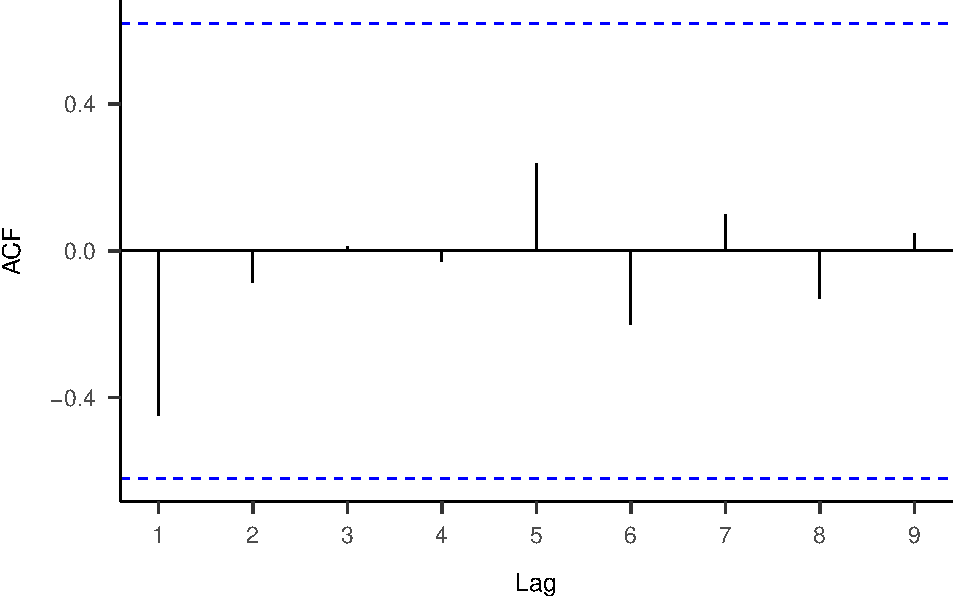
\includegraphics{aggregation_trials_files/figure-latex/acf-joint-high-1.pdf}
\caption{\label{fig:acf-joint-high}Autocorrelations of project acceptance proportions across trials, for the joint presentation high similarity condition. The dashed blue lines represent the 95\% CIs from zero.}
\end{figure}


\end{document}
